\documentclass[a4paper, 12pt]{article}%тип документа



%отступы
\usepackage[left=1cm,right=1cm,top=1cm,bottom=2cm,bindingoffset=0cm]{geometry}

%%% Работа с русским языком
\usepackage{graphicx}
\usepackage{cmap}                           % поиск в PDF
\usepackage{mathtext} 			 	       % русские буквы в формулах
\usepackage[T2A]{fontenc}               % кодировка
\usepackage[utf8]{inputenc}              % кодировка исходного текста
\usepackage[english,russian]{babel} 
\usepackage{float}

\usepackage[export]{adjustbox} % локализация и переносы

\usepackage{subfig}% http://ctan.org/pkg/subfig
\usepackage{booktabs}

\usepackage{wrapfig}


%Матеша
\usepackage{amsmath,amsfonts,amssymb,amsthm,mathtools} % AMS
\usepackage{icomma} % "Умная" запятая

%\mathtoolsset{showonlyrefs=true} % Показывать номера только у тех формул, на которые есть \eqref{} в тексте.

%% Шрифты
\usepackage{euscript}	 % Шрифт Евклид
\usepackage{mathrsfs} % Красивый матшрифт

%% Свои команды
\DeclareMathOperator{\sgn}{\mathop{sgn}}

%% Перенос знаков в формулах (по Львовскому)
\newcommand*{\hm}[1]{#1\nobreak\discretionary{}
	{\hbox{$\mathsurround=0pt #1$}}{}}


%\usepackage{caption}
%\usepackage{subcaption}


\author{Гаврилин Илья Дмитриевич \\
	Б01-101}
\title{\textbf{Работа 3.2.2 \\ 
		Резонанс напряжений в последовательном контуре}}


\begin{document}
	\maketitle
	\section{Аннотация}
	В работе изучили резонанс напряжений в последовательном контуре, изучили резонансные частоты при различных значениях емкости, построили графики ФЧХ и АЧХ, получили значения добротности различными методами.
	\section{Теоретические сведения}
	
	Резонансная частота последовательного контура может быть определена из формулы
	\begin{equation}\label{freq}
		f_r = \frac{1}{2 \pi \sqrt{L C}}.
	\end{equation}
	
	Добротность колебательного контура связана с его параметрами соотношениями:
	\begin{equation}\label{qual}
		Q = \frac{\rho}{R_\Sigma} = \frac{\omega_0 L}{R_\Sigma} = \frac{1}{\omega_0 C R_\Sigma}.
	\end{equation}
	
	Для теоретического расчёта параметров контура используется метод комплексных амплитуд. Импеданс последовательного контура определяется по формуле:
	\begin{equation}\label{импеданс}
		Z = R_\Sigma +i(\omega L - \frac{1}{\omega C}),
	\end{equation}
	где $ R_\Sigma $ -- суммарное активное сопротивление компонентов. $ \omega_0 $ -- резонансная частота контура, при которой импеданс -- действительный. При условии, что $ | \Delta \omega | \ll \omega_0 $, формулы резонансных значений тока и напряжения упрощаются до:
	\begin{equation}\label{Ires}
		\overrightarrow{I} = \frac{E}{R_\Sigma} \frac{\exp i\varphi_I}{\sqrt{1+(\tau \Delta \omega )^2}}, 
	\end{equation}
	\begin{equation}\label{Ures}
		\overrightarrow{U_C} = E Q \frac{\omega_0}{\omega} \frac{\exp i \varphi_C}{\sqrt{1+\tau \Delta \omega )^2}},
	\end{equation}
	где 
	\begin{equation*}
		\varphi_I = -\arctg (\tau \Delta \omega ), 
	\end{equation*}
	\begin{equation}\label{phi_c}
		\varphi_C = -\frac{\pi}{2} + \delta - \arctg (\tau \Delta \varphi ).
	\end{equation}
	Здесь $ \tau = 2 Q / \omega_0 $ -- время затухания колебаний.
	
	Схожесть поведения вблизи резонанса частотных характеристик тока и напряжений на реактивных элементах последовательного контура с добротностью $ Q \gg 1 $ упрощает эксперимент, позволяя проводить измерения именно напряжений.
	
	Резонансное напряжение определяется формулой:
	\begin{equation}\label{resc}
		U_C (\omega_0) \cong Q E
	\end{equation}
	\begin{equation*}
		\varphi_C (\omega_0) = -\frac{\pi}{2}+\delta,
	\end{equation*}
	где $ \delta  $ -- малая поправка.
	
	Заметим, что с одной стороны, $ Q \gg 1 $, так как мы пренебрегаем относительными поправками порядка $ Q^{-2} $, но с другой стороны, в контур встроен резистор для намеренного уменьшения $ Q $, чтобы упростить постройку АЧХ.
	\section{Ход работы}
	\subsection*{Замеры резонансной частоты}
	Следуя пунктам 8, 9 лабораторной работы проведем замеры резонансной частоты и напряжения на конденсаторе в этот момент.\\ \textbf{Замеры для 6 положения тумблера отсутствуют ввиду невозможности его установки переменным конденсатором}
	\begin{table}[H]
		\centering
		\begin{tabular}{|c|c|c|c|c|c|c|c|c|c|c|c|}
			\hline
			$n$ & $C_n$, нФ & \begin{tabular}[c]{@{}c@{}}$f_{0n}$, \\ кГц\end{tabular} & $U_C$, В & $E$, В & \begin{tabular}[c]{@{}c@{}}$L$, \\ мкГн\end{tabular} & $Q$ & \begin{tabular}[c]{@{}c@{}}$\rho$, \\ Ом\end{tabular} & \begin{tabular}[c]{@{}c@{}}$R_{\sum}$, \\ Ом\end{tabular} & \begin{tabular}[c]{@{}c@{}}$R_{S_{\max}}$,\\ Ом\end{tabular} & $R_L$, Ом & $I$, мА \\ \hline
			1 & 24.8 & 32.207 & 4.9738 & 0.1982 & 985.6 & 26 & 326.3 & 12.55 & 0.20 & 8.90 & 0.0080 \\ \hline
			2 & 33.2 & 27.782 & 4.4101 & 0.1982 & 989.4 & 23 & 248.4 & 10.80 & 0.17 & 7.18 & 0.0093 \\ \hline
			3 & 47.6 & 23.245 & 3.8094 & 0.1982 & 985.8 & 22 & 199.5 & 9.07 & 0.14 & 5.47 & 0.0110 \\ \hline
			4 & 57.5 & 21.148 & 3.5141 & 0.1981 & 985.9 & 19 & 157.3 & 8.28 & 0.13 & 4.70 & 0.0121 \\ \hline
			5 & 68.0 & 19.444 & 3.2653 & 0.1982 & 986.2 & 17 & 129.2 & 7.60 & 0.12 & 4.03 & 0.0132 \\ \hline
			6 & 81.6 & -- & -- & -- & -- & -- & -- & -- & -- & -- & -- \\ \hline
			7 & 102.8 & 16.2 & 2.7372 & 0.1980 & 985.4 & 14 & 87.1 & 6.22 & 0.10 & 2.67 & 0.0161 \\ \hline
			\multicolumn{5}{|c|}{Среднее значение} & 986.5 & \multicolumn{4}{c|}{--} & 5.18 & -- \\ \hline
			\multicolumn{5}{|c|}{\begin{tabular}[c]{@{}c@{}}Среднеквадратичная погрешность\\ среднего значения\end{tabular}} & 0.6 & \multicolumn{4}{c|}{--} & 0.83 & -- \\ \hline
			\multicolumn{5}{|c|}{\begin{tabular}[c]{@{}c@{}}Коэффициент Стьюденса\\ $t_{n \alpha}$ для\\ $n = 7$, $\alpha = 0,95$\end{tabular}} & 2.34 & \multicolumn{4}{c|}{--} & 2.34 & -- \\ \hline
			\multicolumn{5}{|c|}{Случайная погрешность} & 3.1 & \multicolumn{4}{c|}{--} & 1.95 & -- \\ \hline
		\end{tabular}
	\end{table}
	\subsection*{Измерение АЧХ}
	Измерим АЧХ для двух положений тумблера конденсатора: для 3 и 5, результаты запишем в таблицу.\\
	\begin{table}[H]
		\centering
		\begin{tabular}{|ccc|ccc|}
			\hline
			\multicolumn{3}{|c|}{С=47.6 нФ}                                        & \multicolumn{3}{c|}{С=68.0 нФ}                                        \\ \hline
			\multicolumn{1}{|c|}{f, kГц} & \multicolumn{1}{c|}{Uc, В}     & E, В      & \multicolumn{1}{c|}{f, kГц} & \multicolumn{1}{c|}{Uc, В}     & E, В      \\ \hline
			\multicolumn{1}{|c|}{22.37}  & \multicolumn{1}{c|}{2.0403} & 0.1968 & \multicolumn{1}{c|}{18.571} & \multicolumn{1}{c|}{1.8138} & 0.2031 \\ \hline
			\multicolumn{1}{|c|}{22.565} & \multicolumn{1}{c|}{2.458}  & 0.1967 & \multicolumn{1}{c|}{18.751} & \multicolumn{1}{c|}{2.114}  & 0.2032 \\ \hline
			\multicolumn{1}{|c|}{22.82}  & \multicolumn{1}{c|}{2.855}  & 0.197  & \multicolumn{1}{c|}{19.008} & \multicolumn{1}{c|}{2.669}  & 0.2033 \\ \hline
			\multicolumn{1}{|c|}{22.977} & \multicolumn{1}{c|}{3.43}   & 0.1968 & \multicolumn{1}{c|}{19.243} & \multicolumn{1}{c|}{3.1804} & 0.2034 \\ \hline
			\multicolumn{1}{|c|}{23.253} & \multicolumn{1}{c|}{3.7784} & 0.197  & \multicolumn{1}{c|}{19.523} & \multicolumn{1}{c|}{3.3135} & 0.2033 \\ \hline
			\multicolumn{1}{|c|}{23.5}   & \multicolumn{1}{c|}{3.4991} & 0.1967 & \multicolumn{1}{c|}{19.737} & \multicolumn{1}{c|}{2.996}  & 0.2031 \\ \hline
			\multicolumn{1}{|c|}{23.754} & \multicolumn{1}{c|}{2.9572} & 0.1965 & \multicolumn{1}{c|}{19.995} & \multicolumn{1}{c|}{2.4756} & 0.2029 \\ \hline
			\multicolumn{1}{|c|}{24.064} & \multicolumn{1}{c|}{2.346}  & 0.1962 & \multicolumn{1}{c|}{20.221} & \multicolumn{1}{c|}{2.0747} & 0.2027 \\ \hline
			\multicolumn{1}{|c|}{24.266} & \multicolumn{1}{c|}{2.0231} & 0.1962 & \multicolumn{1}{c|}{20.605} & \multicolumn{1}{c|}{1.573}  & 0.2026 \\ \hline
			\multicolumn{1}{|c|}{24.508} & \multicolumn{1}{c|}{1.718}  & 0.1962 & \multicolumn{1}{c|}{--}       & \multicolumn{1}{c|}{--}      &    --  \\ \hline
		\end{tabular}
		\caption{АЧХ для последовательного контура при различных значениях емкости}
	\end{table}
	По полученным данным построим АЧХ, после нормализуем ее для оценки добротности системы.\\
	\begin{figure}[H]
		\centering
		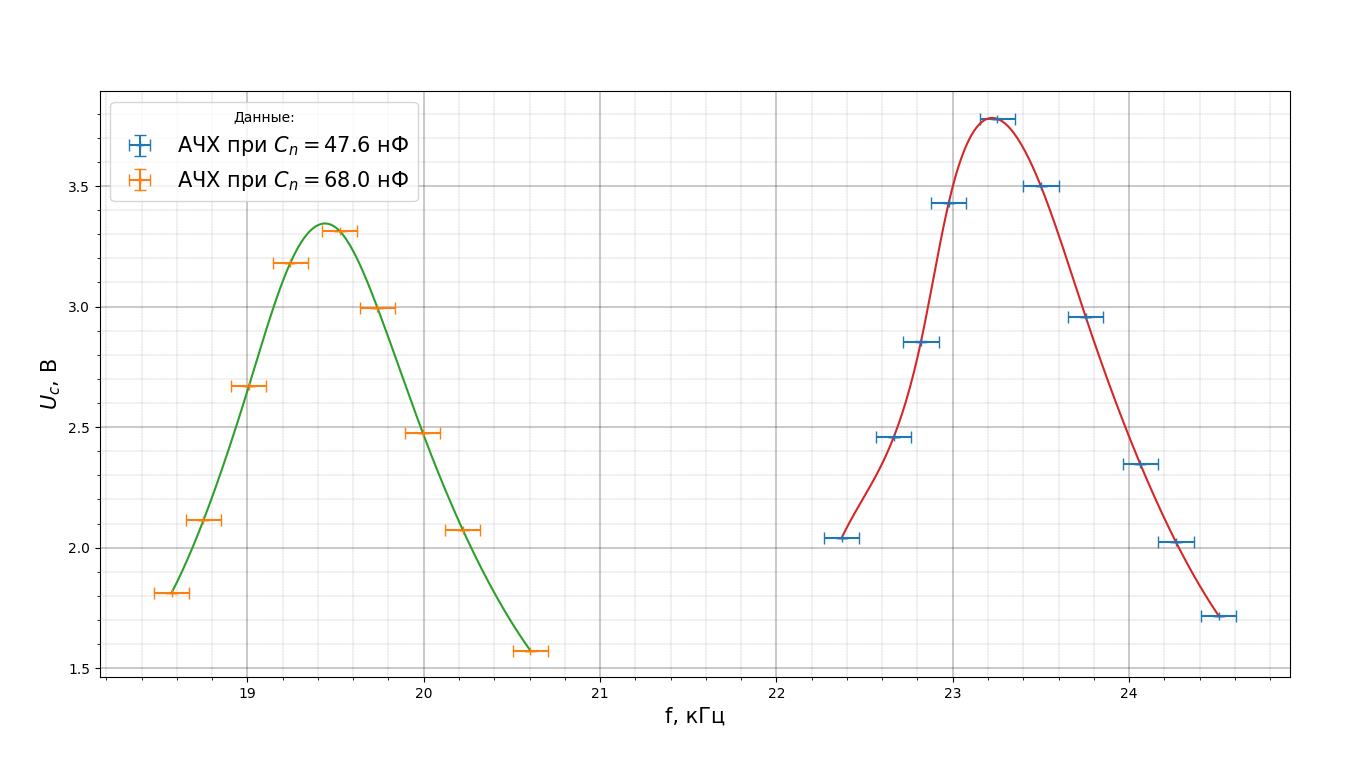
\includegraphics[width=0.92\linewidth]{ачх}
		\caption{АЧХ последовательного контура}
		\label{fig:}
	\end{figure}
	По нормализованному графику оценим добротность колебательной системы. Проведем линию на уровне 0.707 и замерим ширину АЧХ. $Q_3 = 21 \pm 8; Q_5 = 15 \pm 6$. Получили значения сходные с рассчитанными ранее.
	\begin{figure}[H]
		\centering
		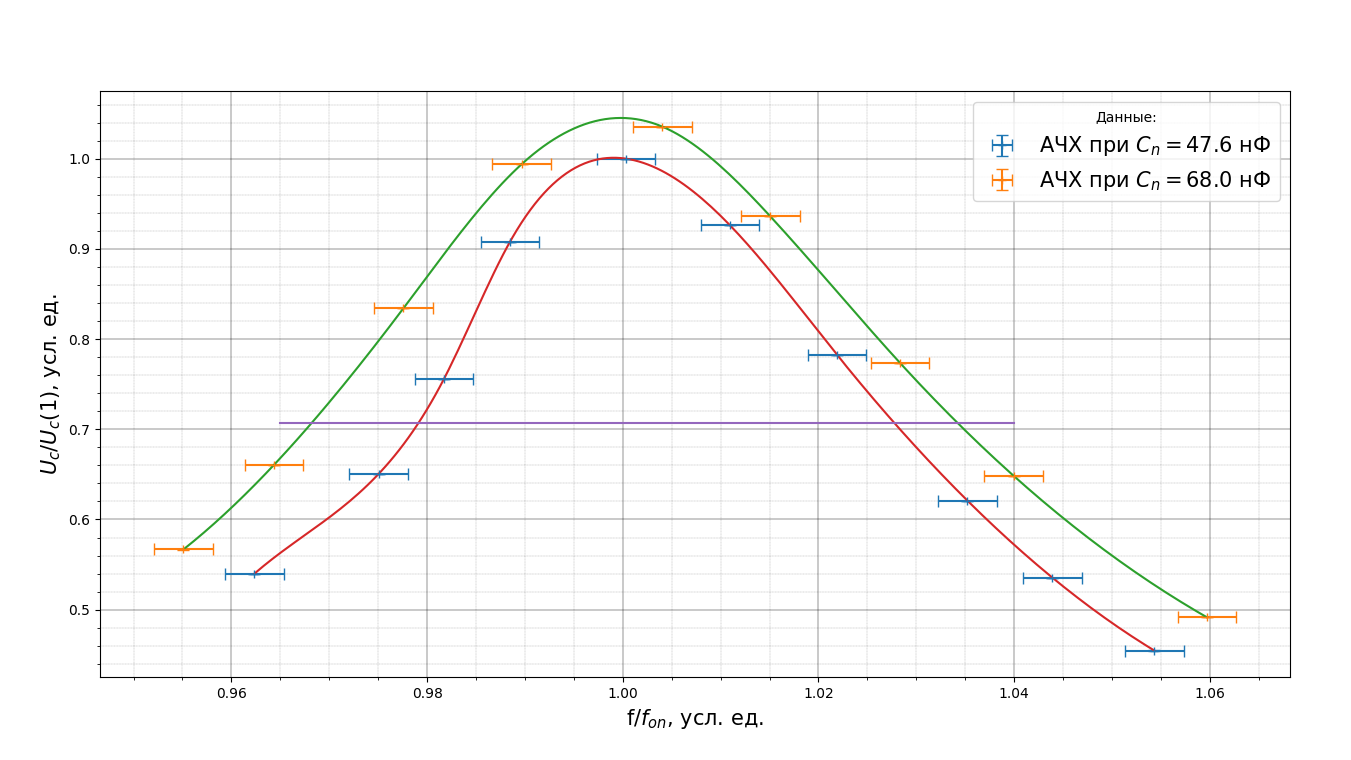
\includegraphics[width=0.92\linewidth]{ачх_норм}
		\caption{Нормализованное АЧХ последовательного контура}
		\label{fig:}
	\end{figure}
	\subsection*{Фазо-частотная характеристика}
	\begin{table}[H]
		\centering
		\begin{tabular}{|ccc|ccc|}
			\hline
			\multicolumn{3}{|c|}{$С_n=102.8$   нФ}                            & \multicolumn{3}{c|}{$С_n=33.2$ нФ}                               \\ \hline
			\multicolumn{1}{|c|}{f, kГц} & \multicolumn{1}{c|}{x}   & $x_0$ & \multicolumn{1}{c|}{f, kГц} & \multicolumn{1}{c|}{x}   & $x_0$ \\ \hline
			\multicolumn{1}{|c|}{13.646} & \multicolumn{1}{c|}{0.3} & 4   & \multicolumn{1}{c|}{25.758} & \multicolumn{1}{c|}{0.3} & 3.9 \\ \hline
			\multicolumn{1}{|c|}{13.808} & \multicolumn{1}{c|}{0.3} & 4   & \multicolumn{1}{c|}{26.015} & \multicolumn{1}{c|}{0.4} & 3.9 \\ \hline
			\multicolumn{1}{|c|}{14.043} & \multicolumn{1}{c|}{0.3} & 3.9 & \multicolumn{1}{c|}{26.237} & \multicolumn{1}{c|}{0.4} & 3.8 \\ \hline
			\multicolumn{1}{|c|}{14.258} & \multicolumn{1}{c|}{0.4} & 3.9 & \multicolumn{1}{c|}{26.502} & \multicolumn{1}{c|}{0.5} & 3.8 \\ \hline
			\multicolumn{1}{|c|}{14.522} & \multicolumn{1}{c|}{0.4} & 3.9 & \multicolumn{1}{c|}{26.714} & \multicolumn{1}{c|}{0.6} & 3.8 \\ \hline
			\multicolumn{1}{|c|}{14.728} & \multicolumn{1}{c|}{0.5} & 3.9 & \multicolumn{1}{c|}{27.036} & \multicolumn{1}{c|}{0.7} & 3.7 \\ \hline
			\multicolumn{1}{|c|}{15.021} & \multicolumn{1}{c|}{0.6} & 3.2 & \multicolumn{1}{c|}{27.253} & \multicolumn{1}{c|}{0.9} & 3.7 \\ \hline
			\multicolumn{1}{|c|}{15.241} & \multicolumn{1}{c|}{0.8} & 3.3 & \multicolumn{1}{c|}{27.488} & \multicolumn{1}{c|}{1.2} & 3.7 \\ \hline
			\multicolumn{1}{|c|}{15.498} & \multicolumn{1}{c|}{1.1} & 3.3 & \multicolumn{1}{c|}{27.763} & \multicolumn{1}{c|}{1.7} & 3.7 \\ \hline
			\multicolumn{1}{|c|}{15.811} & \multicolumn{1}{c|}{1.6} & 3.2 & \multicolumn{1}{c|}{28.094} & \multicolumn{1}{c|}{1.3} & 3.6 \\ \hline
			\multicolumn{1}{|c|}{15.995} & \multicolumn{1}{c|}{1.8} & 3.1 & \multicolumn{1}{c|}{28.201} & \multicolumn{1}{c|}{1.4} & 3.6 \\ \hline
			\multicolumn{1}{|c|}{16.236} & \multicolumn{1}{c|}{1.2} & 3.1 & \multicolumn{1}{c|}{28.573} & \multicolumn{1}{c|}{2.7} & 3.6 \\ \hline
			\multicolumn{1}{|c|}{16.552} & \multicolumn{1}{c|}{1.4} & 3   & \multicolumn{1}{c|}{28.826} & \multicolumn{1}{c|}{2.8} & 3.5 \\ \hline
			\multicolumn{1}{|c|}{16.761} & \multicolumn{1}{c|}{2.4} & 3   & \multicolumn{1}{c|}{29.087} & \multicolumn{1}{c|}{2.9} & 3.5 \\ \hline
			\multicolumn{1}{|c|}{17.078} & \multicolumn{1}{c|}{2.5} & 3   & \multicolumn{1}{c|}{--}       & \multicolumn{1}{c|}{--}    &   --  \\ \hline
			\multicolumn{1}{|c|}{17.331} & \multicolumn{1}{c|}{2.5} & 2.9 & \multicolumn{1}{c|}{--}       & \multicolumn{1}{c|}{--}    &  --   \\ \hline
			\multicolumn{1}{|c|}{18.278} & \multicolumn{1}{c|}{2.5} & 2.8 & \multicolumn{1}{c|}{--}       & \multicolumn{1}{c|}{--}    &  --   \\ \hline
		\end{tabular}
	\caption{Зависимость сдвига фазы от частоты в последовательном контуре}
	\end{table}
	Замерим зависимость фазы от частоты для последовательного контура, отнормируем координаты, построим требуемый график.\\
	\begin{figure}[H]
		\centering
		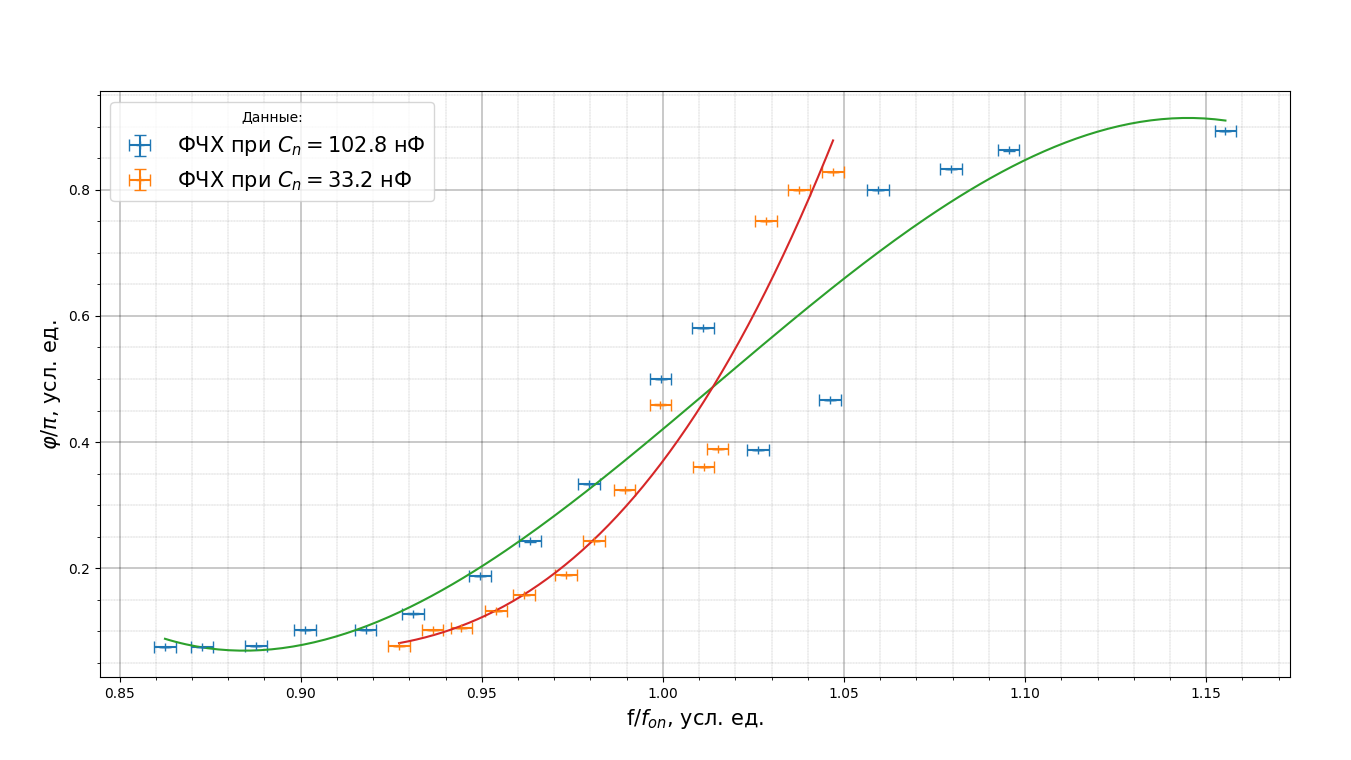
\includegraphics[width=0.92\linewidth]{фчх}
		\caption{Нормализованное ФЧХ последовательного контура}
		\label{fig:}
	\end{figure}
	С помощью данных замеров рассчитаем добротность контура: $Q_7=13 \pm 4; Q_2 = 24 \pm 7$.\\
	Также построим зависимость $R_L$ от частоты.\\
	\begin{figure}[H]
		\centering
		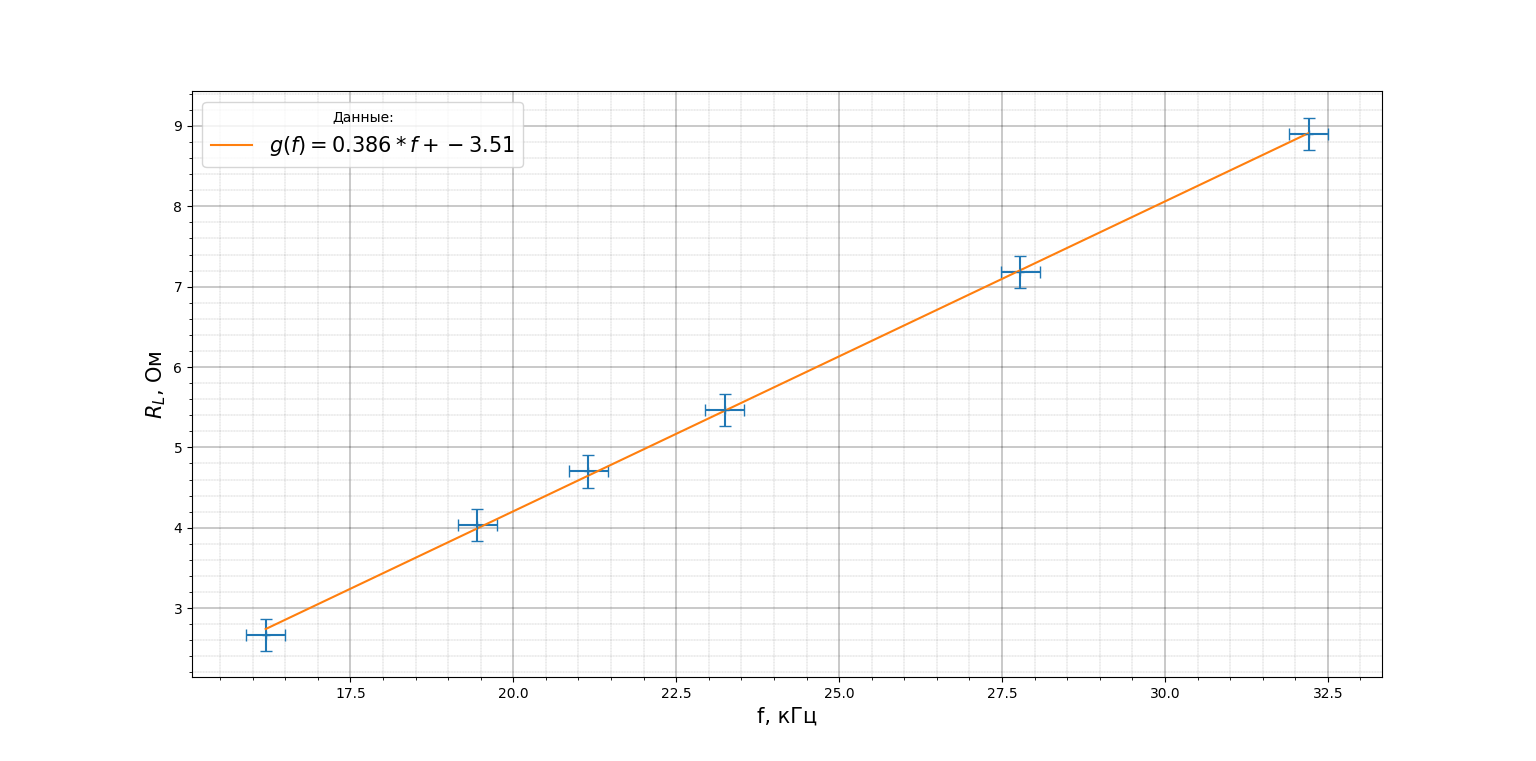
\includegraphics[width=0.92\linewidth]{rl}
		\caption{Зависимость $R_L$ от $f_{0n}$}
		\label{fig:rl}
	\end{figure}
	
	\section{Выводы}
	1) В работе изучили резонанс напряжения в последовательном контуре, получили значения резонансных частот и напряжение на конденсаторе в этот момент.\\
	2) Замерили ФЧХ и АЧХ для этого контура, по графикам характеристик получили значения добротности. \\
	3) При всех способах измерения добротности получили сходные значения добротности, что говорит о справедливости всех методов измерения.\\
\end{document}